\subsection*{Aufgabe 3}

(Klausur WS 2011/12) In einer Umfrage wurden 500 Studierende der HS Regensburg
(darunter 300 M�nner und 200 Frauen) nach ihrer Zufriedenheit mit dem Studium an der
Hochschule gefragt. \newline

Die folgende Kreuztabelle zeigt die erhaltenen Antworth�ufigkeiten:

\begin{center}
\begin{figure}[!htbp]
\fbox{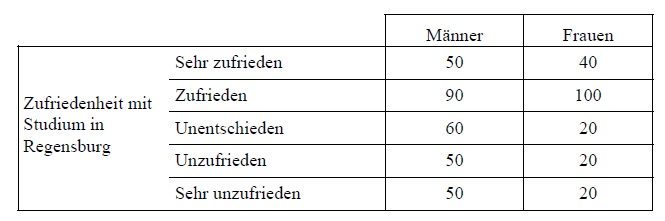
\includegraphics[width=0.9\textwidth,page=1]{chapters_AB/Grafiken_AB/AB_2_3.jpg}} 
\end{figure}
\end{center}

\begin{enumerate}[label=\alph*)]
\item Berechnen Sie die bedingten Verteilungen (relative H�ufigkeiten) der Zufriedenheit unter den M�nnern bzw. den Frauen. W�hlen Sie jeweils einen beliebigen Wert aus jeder der
beiden bedingten Verteilungen, und beschreiben Sie in jeweils einem Satz, was diese
Zahlen inhaltlich aussagen.
\vspace{5cm}
\item Sind die beiden Merkmale statistisch unabh�ngig? Wenn nein: wie m�sste die Kreuztabelle bei Unabh�ngigkeit aussehen, wenn die Randverteilungen mit denen der obigen Tabelle �bereinstimmen sollen?
\newpage
\item Zeichnen Sie (nebeneinander) Box-Plots f�r die beiden bedingten Verteilungen aus a)!
Kodieren Sie dazu die Zufriedenheit mit den ganzen Zahlen von 1 bis 5!
\end{enumerate}